% ============================================================
% UGA-Themed Beamer Template (Clean MWE)
% ============================================================

\documentclass[aspectratio=169,professionalfonts]{beamer}

% ---------- COLORS (swap with official UGA hex if you like) ----------
\usepackage{xcolor}
\definecolor{UGARed}{HTML}{BA0C2F}   % Verify with brand guide
\definecolor{UGABlack}{HTML}{000000}
\definecolor{UGAGray}{HTML}{8A8D8F}

% ---------- THEME & PROGRESS DOTS ----------
\usetheme{default}
\useinnertheme{circles}
\useoutertheme[subsection=false]{miniframes} % dots across top
\usefonttheme{professionalfonts}
\setbeamertemplate{navigation symbols}{}
% Head/foot colors
\setbeamercolor{subsection in head/foot}{fg=white,bg=UGARed}
\setbeamercolor{headline}{fg=white, bg=UGARed}

\setbeamercolor{section in head/foot}{fg=white,bg=UGARed}
\setbeamercolor{section in head/foot shaded}{fg=white,bg=white}
\setbeamercolor{footline}{bg=UGABlack,fg=white}
\setbeamercolor{frametitle}{fg=UGABlack}
\setbeamercolor{title}{fg=UGABlack}
\setbeamercolor{normal text}{fg=UGABlack}
\setbeamercolor{structure}{fg=UGARed}

% --- HEADLINE: miniframes-style dots with your colors ---
\setbeamertemplate{headline}{
  \begin{beamercolorbox}[wd=\paperwidth,ht=2.5ex,dp=1.125ex]{headline}
    \insertsectionnavigationhorizontal{\paperwidth}{}{}
  \end{beamercolorbox}
}

% Optional: keep unselected items faint (works fine with miniframes)

% Simple footline with slide numbers
\setbeamertemplate{footline}{
  \leavevmode%
  \hbox{%
    \begin{beamercolorbox}[wd=\paperwidth,ht=2.5ex,dp=1ex,leftskip=1em,rightskip=1em]{footline}%
      \insertshortauthor{} \hfill \insertframenumber/\inserttotalframenumber
    \end{beamercolorbox}}%
}

% ---------- PACKAGES ----------
\usepackage{amsmath,amssymb,mathtools}
\usepackage{graphicx}
\usepackage{booktabs}
\usepackage{array}
\usepackage{adjustbox}
\usepackage{hyperref}
\usepackage{tikz}
\usetikzlibrary{arrows.meta, positioning}
\usepackage{tcolorbox}
\usepackage{eurosym}
\usepackage{threeparttable}
% ---------- METADATA (fill these later) ----------
\title[Taxation and International Migration of Superstars]{Evidence from the European Football Market}
\subtitle{Henrik Jacobsen Kleven, Camille Landais and Emmanueal Saez}
\author[Tate Mason]{Tate Mason}
\institute[UGA]{John Munro Godfrey Sr. Dept. of Economics \\ University of Georgia}
\date{\today}

% ---------- AUTO-AGENDA EACH SECTION ----------
\AtBeginSection[]{
  \begin{frame}{Roadmap}
    \tableofcontents[currentsection]
  \end{frame}
}

% ---------- MACROS ----------
% Numbered equation with label
\newcommand{\beq}[1]{\begin{equation}\label{#1}}
\newcommand{\eeq}{\end{equation}}
% Accent color highlight
\newcommand{\hl}[1]{\textbf{\textcolor{UGARed}{#1}}}
% Simple figure placeholder macro
\newcommand{\figph}[2][0.9\linewidth]{%
  \begin{figure}
    \centering
    \fbox{\rule{0pt}{0.55#1}\rule{#1}{0pt}}%
    \caption{#2}
  \end{figure}
}

% ============================================================

% ===== Added helper macros for talk version =====
\usepackage{booktabs, adjustbox}
\usepackage{amsmath, amssymb}
\usepackage{graphicx}
\usepackage{hyperref}
\hypersetup{colorlinks=true, linkcolor=UGARed, urlcolor=UGARed}

% Subtle highlight macro
\newcommand{\hl}[1]{\textbf{\color{UGARed}{#1}}}

% Figure/table placeholder
\newcommand{\figph}[1]{\begin{center}\fbox{\parbox{0.85\linewidth}{\centering \vspace{0.6em} \textit{#1} \vspace{0.6em}}}\end{center}}


\begin{document}

% ------------------------------------------------------------
% Title
% ------------------------------------------------------------
\begin{frame}
  \titlepage
  % TALK GOAL: Speak ~45 minutes. Slides are intentionally concise.
  % Use Notes or presenter view for your speaking points.
\end{frame}
% ============================================================
\section{Motivation \& Background}
% ============================================================

\begin{frame}{Question \& Motivation}
  \begin{itemize}
    \item \hl{Question:} How do favorable tax policies induce migration for high-skilled individuals?
    \item Using data which tracks footballers' movement across leagues and countries, how did tax policies in Spain and Denmark affect migration decisions?
    \item Find notable shifts in demographic makeups of national leagues following policy changes, indicating that favorable policy leads to an influx of high skilled labor.
  \end{itemize}
\end{frame}

\begin{frame}{Why Football?}
  \begin{itemize}
    \item Football contracts and by extension, movements, are easily tracable given it is a profession which is for entertainment
    \item Footballers at an elite level are certainly in the top end of the income distribution, thus leading them to be directly impacted by a tax cut for high skilled labor
    \item Football specific policy (Bosman Rule) provides another source of mobility variation, allowing for analysis of tax policy at multiple phases in the "football life cycle"
  \end{itemize}
\end{frame}

\begin{frame}{Contribution}
  \begin{itemize}
    \item \hl{What’s new}: Implements a novel dataset of high-earning, high-skilled laborers' mobility patterns
    \item \hl{Why it matters}: Allows for analysis of cross-country migration in the face of tax policy changes
  \end{itemize}
\end{frame}

% =========================================================
\section{Mirrleesian Framwork}
% =========================================================

\begin{frame}{Overview}
  \begin{itemize}
    \item 1981 Paper: "Migration and Optimal Income Taxes"
    \item How to optimally tax citizens earning income abroad as to reduce waste
    \item How do taxes impact the distribution of agents?
    \item How do taxes play as incentives for agents?
  \end{itemize}
\end{frame}

\begin{frame}{Model Considerations}
  \begin{tcolorbox}[colback=red!5!white,colframe=red!75!black]
    The three criteria concerning migration research, according to Mirrlees
  \end{tcolorbox}
  \begin{enumerate}
    \item Restriction to the group who does not migrate
    \begin{itemize}
      \item Suboptimal as this does not account for those who wished to move but were constrained
      \item Misses those who leave and still contribute to their country, a group which countries do not appear to be too concerned with
      \item Restriction of taxes and corresponding benefits to voters, a confusing group as there are various definitions of voters
    \end{itemize}
    \item Definition of "Nationals"
    \begin{itemize}
      \item Overly restrictive and presumptuous (i.e. exclusion of immigrants)
    \end{itemize}
    \item All humans
    \begin{itemize}
      \item Not realistic as this definition would neglect welfare of the citizens of other countries
    \end{itemize}
  \end{enumerate}
\end{frame}

\begin{frame}{Foreign-Income Tax Model}
  \begin{itemize}
    \item Consumer utility: $u(x, y, y', z, n)$
    \item Tax policy of the domestic government: $x = c(y, z) + y'$
    \item Foreign Income is taxed at a higher marginal tax rate than domestic when:
    \begin{gather*}
      \frac{\partial}{\partial n}\frac{u_y(x, y, z, n)}{u_z(x, y, z, n)} < 0
    \end{gather*}
    \begin{itemize}
      \item note: case when untaxed foreign earnings $y'$ are not present 
    \end{itemize}
  \end{itemize}
\end{frame}

\begin{frame}{Model, cont.}
  \begin{itemize}
    \item When introducing $y'$, agent chooses value to maximize:
    \begin{gather*}
      u(c(y, z) + y', y, y', z, n)
    \end{gather*}
    \item Envelope theorem yields:
    \begin{gather*}
      \bar{u}_y = u_y(c+y', y, y', z, n) \\
      \bar{u}_z = u_z(c + y', y, y', z, n)
    \end{gather*}
    \begin{gather*}
      s(c,y,y',z,n) = \frac{u_y}{u_z} \\ 
      \shortintertext{such that foreign income is taxed higher at the margin if:}
      s_n + s_{y'}\frac{\partial y'}{\partial n} > 0
    \end{gather*}
    \item note: $s$ is willingness to substitute domestic and foreign earnings
    \item $n$ and $y'$ play opposition to each other on $s$, with $s_n<0$ and $s_{y'}>0$
    \item Implies that a lower marginal tax rate on domestic income is reasonable with $y'$
  \end{itemize}
\end{frame}

\begin{frame}{Connecting to Kleven et. al}
  \begin{itemize}
    \item Use this type of model to show how migration patterns vary by ability level of footballers
    \item Takes exogenous policy changes as opportunity to test intuition provided by model
    \item More concerned with migration responses to the tax policy than defining optimal policy
  \end{itemize}
\end{frame}

% ============================================================
\section{Institutional Framework}
% ============================================================

\begin{frame}{International Football, an Overview}
  \begin{itemize}
    \item Football in Europe is a behemoth: 50+ leagues, 21,000 players
    \item Top Five Leagues: England, Spain, Germany, Italy, France
    \item \euro 20.4bn in revenue from Top Five alone
    \begin{tcolorbox}[colback=red!5!white,colframe=red!75!black]
      Massive Player Transfer Market - \euro 11bn in 2025
    \end{tcolorbox}
  \end{itemize}
\end{frame}

\begin{frame}{The Transfer Market}
  \begin{itemize}
    \item Teams pay to purchase rights to players' services
    \item Two windows:
    \begin{enumerate}
      \item Summer: June - September 1, seen as main window
      \item Winter: January
    \end{enumerate}
    \item System allows for player movement to be easily followed
    \item Contract numbers are commonly recorded, with approximations easily accessible
  \end{itemize}
\end{frame}

\begin{frame}{An Example of Transfers}
  \begin{itemize}
    \item In 2025, Liverpool F.C. spent \euro 520m during the summer breaking the Premier League record for most expensive transfer twice
    \item Importantly, not one of the seven incoming players are English or British
    \item In Liverpool's last match (at time of writing), they did not start a single British player, with only two senior British players being in the larger squad (20 players)
    \item How is this possible?
  \end{itemize}
\end{frame}

% ============================================================
\section{Kleven, Landais, Saez - Introduction}
% ============================================================

\begin{frame}{What is Their Goal?}
  \begin{itemize}
    \item How does variation in top tax rates affect the migration of footballers in Europe?
    \item Exploit variation across multiple dimensions:
    \begin{enumerate}
      \item Variation in top tax rates across countries and over time
      \item Preferential taxation schemes in specific countries
      \item Bosman Rule
    \end{enumerate}
    \item Utilize a Mirrleesian theoretical framework applied to a multinomial logit to determine player choices
  \end{itemize}
\end{frame}

\begin{frame}{Policy Overview - Bosman}
  \begin{itemize}
    \item Bosman ruling occurred in 1995, overhauling much of the football status quo
    \item Prior to Bosman ruling:
    \begin{enumerate}
      \item Three-player rule: no more than three foreign players per team could participate in any game in UEFA club competitions
      \item Transfer-fee rule: require a transfer fee even when a player became a free agent
    \end{enumerate}
    \item Bosman posed as a major hurdle to mobility both domestically and across countries
    \item Note: Foreign-player rule was still in some sort of effect, applying to non-Europeans after 1995
  \end{itemize}
\end{frame}

\begin{frame}{Policy Overview - Top Tax Schema}
  \hl{Spain}:
  \begin{itemize}
    \item Beckham law: Flat tax of 24\% for foreign workers relocating to Spain after Jan. 1, 2004
    \item Reduction from 45\% at time of passing
    \item Can not have been a taxable resident of Spain in any of the preceding 10 years to be eligible
  \end{itemize}
  \hl{Denmark}:
  \begin{itemize}
    \item Researchers' Tax Scheme: Flat tax of 25\% for high income foreigners signing for employment in Denmark after June 1, 1991
    \item Reduction from 68\% top tax rate at time of introduction
    \item Can not have been tax liable to Denmark for 3 years prior to scheme and must make at least \euro 103,000
  \end{itemize}
\end{frame}

% ============================================================
\section{Theoretical Model}
% ============================================================

\begin{frame}{Baseline Model - Flexible Demand}
  \begin{itemize}
    \item $\exist \ N = \{n_1, n_2, \cdots, c_N\}$ countries possessing a continuum of domestic potential players
    \item Each player is endowed with footballing ability $a\geq0$
    \item If they play, the agent generates value $a$ for their club
    \item As in Mirrlees, before-tax wage is equal to ability, $a$
  \end{itemize}
\end{frame}
\begin{frame}{Baseline Model, cont.}
  \begin{itemize}
    \item Player also assigned country of origin $m$ and preferences $\mu_m = (\mu_{1m}, \mu_{2m}, \cdots, \mu_{Nm})$ for each location
    \item A player thus gets utility from country $n$ by
    \begin{gather*}
      u(a(1-\tau_{nm})) + \mu_{nm}
    \end{gather*}
    \item where $u(\cdot)$ is increasing and $\tau_{nm}$ is the tax rate in $n$ for a player from $m$
    \item IC condition is thus
    \begin{gather*}
      u(a(1-\tau_{nm})) + \mu_{nm} \geq \max_{n'}\{u(a(1-\tau_{n'm})) + \mu_{n'm}
    \end{gather*}
  \end{itemize}
\end{frame}
\begin{frame}{Baseline Model, cont.}
  \begin{itemize}
    \item Define $g_m(\mu_m, a)$ as the joint distribution of players from $m$ with ability $a$ playing in $n$
    \item This measure of player supply is denoted as $p_{nma}$ henceforth
    \item Total Measure of players in country $n$ from country $m$ with any ability level as 
    \begin{gather*}
      p_{nm}(1-\tau_{nm}) \equiv \int\limits_0^{\infty}p_{nma}(a(1-\tau_{nm}))da
    \end{gather*}
  \end{itemize}
\end{frame}
\begin{frame}{Baseline Model, cont.}
  \begin{itemize}
    \item Countries may seperate tax rates such that $\tau_{nn} = \tau_{nd}$ and $\tau_{nm} = \tau_{nf}$ $\forall \ n\ne m$
    \item Distributions by foreign and domestic can be defined as 
    \begin{gather*}
      \shortintertext{Domestic:}
      p_{nd}(1-\tau_{nd})\equiv\int\limits_0^{\infty}p_{nda}(a(1-\tau_{nd}))da \\
      \shortintertext{Foreign:}
      p_{nf}(1-\tau_{nf})\equiv\int\limits_0^{\infty}p_{nfa}(a(1-\tau_{nf}))da
    \end{gather*}
  \end{itemize}
\end{frame}
\begin{frame}{Baseline Model, cont.}
  \hl{Proposition 1:}
  \begin{tcolorbox}[colback=red!5!white,colframe=red!75!black]
    Assuming that density $g_m(\mu_m, a)$ is smooth and positive everywhere on domain D, $p_{nda}, p_{nfa} > 0$
    for all $n, a$ and
    \begin{enumerate}
      \item $p_{nda}$ is decreasing in $\tau_{nd}$ and unaffected by $\tau_{nf}$
      \item $p_{nfa}$ is decreasing in $\tau_{nf}$ and unaffected by $\tau_{nd}$
    \end{enumerate}
  \end{tcolorbox}
  \begin{itemize}
    \item States own-tax effect on number of both types of player is negative at all abilities
    \item Cross-tax effect is zero
  \end{itemize}
\end{frame}
\begin{frame}{Baseline Model, cont.}
  \begin{itemize}
    \item Denote elasticities of players in a country $n$ w.r.t. net-of-tax rate on players in country $n$
    \begin{gather*}
      \shortintertext{Foreign:}
      \varepsilon_{nf} = \frac{dp_{nf}}{d(1-\tau_{nf})}\frac{1-\tau_{nf}}{p_{nf}} \\
      \shortintertext{Domestic:}
      \varepsilon_{nd} = \frac{dp_{nd}}{d(1-\tau_{nd})}\frac{1-\tau_{nd}}{p_{nd}} \\
    \end{gather*}
    \item Given approx. 85-90 percent of players are domestic, cutting rates on only foreign players can attract a large number of new players while having meager effects on preexisting foreign players
  \end{itemize}
\end{frame}

\begin{frame}{Adding Rigid Demand}
  \hl{Assumptions}
  \begin{itemize}
    \item Assume each country's football market hires a continuum of measure one of players
    \item Players are hired by a continuum of clubs of measure one (each club hires one player)
    \item No new entry by clubs
    \item Population of potential native players in a country $n$ has measure $P_n > 1$, meaning not all players can play in equilibrium
    \item Non-players work in a regular labor market with wage set to zero
  \end{itemize}
\end{frame}
\begin{frame}{Rigid Demand, cont.}
  \hl{Lemma 1:}
  \begin{tcolorbox}[colback=red!5!white,colframe=red!75!black]
    In any equilibrium, within any country $n$, surplus $s_n\geq0$ captured by each club is constant across all clubs and players in said country.
    Thus, before-tax wage paid out to a player of ability $a$ in country $n$ is $a-s_n$. No player with $a < s_n$ plays in country $n$.
  \end{tcolorbox}
  \begin{itemize}
    \item Form follows as before, except for before-tax income now being $a-s_n$
  \end{itemize}
\end{frame}
\begin{frame}{Rigid Demand, cont.}
  \begin{itemize}
    \item Total number of players in a country $n$ across ability levels is now represented as
    \begin{gather*}
      \shortintertext{Domestic:}
      p_{nd}(s_n, 1-\tau_{nd}) \equiv \int\limits_{s_n}^{\infty}p_{nda}((a-s_n)(1-\tau_{nd})) \\
      \shortintertext{Foreign:}
      p_{nf}(s_n, 1-\tau_{nf}) \equiv \int\limits_{s_n}^{\infty}p_{nfa}((a-s_n)(1-\tau_{nf})) \\
    \end{gather*}
    \item Both functions decrease in $s_n$, but $p_{ni}$ is increasing in $(1-\tau_{ni})$ for $i = (f,d)$
  \end{itemize}
\end{frame}
\begin{frame}{Rigid Demand, cont.}
  \begin{itemize}
    \item Only general equilibrium differs, requiring
    \begin{gather*}
      p_{nd}(s_n,1-\tau_{nd}) + p_{nf}(s_n, 1-\tau_{nf}) = 1 \\
      \Rightarrow s_n = s_n(1-\tau_{nd}, 1-\tau_{nf})
    \end{gather*}
    \item By inserting equilirbium surplus into $p_{nd}, p_{nda}, p_{nf}, p_{nfa}$, obtain relationships which are functions of tax rates
  \end{itemize}
\end{frame}
\begin{frame}{Rigid Demand, cont.}
  \hl{Proposition 2:}
  \begin{tcolorbox}[colback=red!5!white,colframe=red!75!black]
    Assume that countries are small and that density $g_m(\mu_m, a)$ is smooth and positive everywhere on its domain $D$. Then, $p_{nda}, p_{nfa}>0$ for all $a > s_n$, and:
    \begin{enumerate}
      \item $s_n(1-\tau_{nd}, 1-\tau_{nf})$ decreases with $\tau_{nd} \ \text{and} \ \tau_{nf}$
      \item $p_{nda}(1-\tau_{nd}, 1-\tau_{nf})$ decreases with $\tau_{nd}$ at high abilities, increases with $\tau_{nd}$ at low abilities, and increases with $\tau_{nf}$ at all abilities
      \item $p_{nfa}(1-\tau_{nd}, 1-\tau_{nf})$ decreases with $\tau_{nf}$ at high abilities, increases with $\tau_{nf}$ at low abilities, and increases with $\tau_{nd}$ at all abilities
      \item $p_{nd}(1-\tau_{nd}, 1-\tau_{nf})$ decreases with $\tau_{nd}$ and increases with $\tau_{nf}$
      \item $p_{nf}(1-\tau_{nd}, 1-\tau_{nf})$ decreases with $\tau_{nf}$ and increases with $\tau_{nd}$
    \end{enumerate}
  \end{tcolorbox}
\end{frame}
\begin{frame}{Discussion of Model}
  \begin{itemize}
    \item Sorting effects related to own-tax and cross-tax effects:
    \begin{enumerate}
      \item Taxing foreign players no reduces the number of foreign players at all ability levels
      \item Due to equilibrium sorting, there is now a cross-tax effect of taxing one group on the other
    \end{enumerate}
    \item High ability players have $a \gg s_n$ such that $a - s_n \simeq a$ (response to taxation is basically the same in both specifications), thus mobility elasticity for high-ability players is the upper bound relevant for other high-income occupations with flexible labor demand
  \end{itemize}
  \end{frame}

% ============================================================
\section{Reduced Form Results}
% ============================================================

\begin{frame}{Bosman Ruling Cross-Country Correlations}
  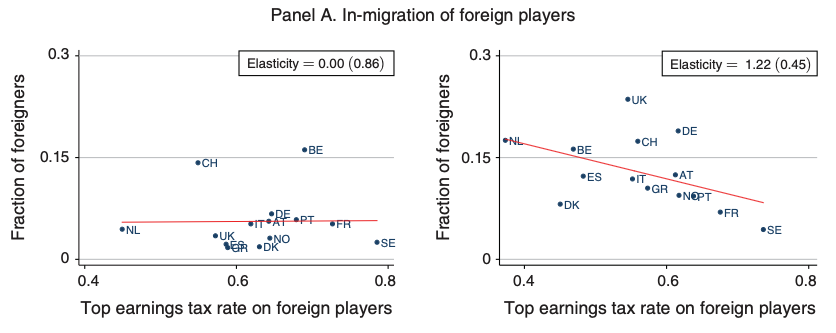
\includegraphics[
    width = \textwidth,
    keepaspectratio
  ]{bosman_1a.png}
\end{frame}

\begin{frame}{Bosman Ruling Cross-Country Correlations}
  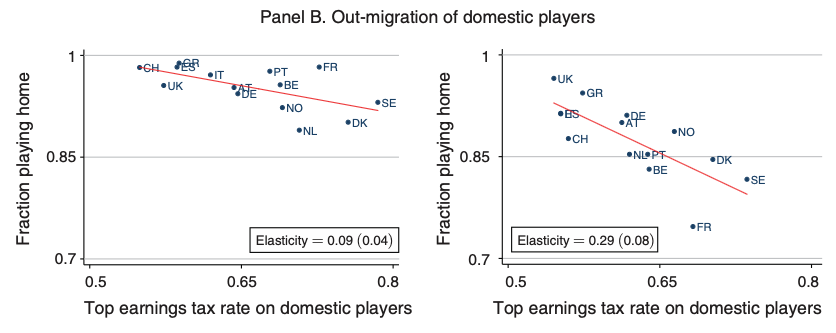
\includegraphics[
    width = \textwidth,
    keepaspectratio
  ]{bosman_1b.png}
\end{frame}

\begin{frame}{Bosman Ruling Cross-Country Correlations}
  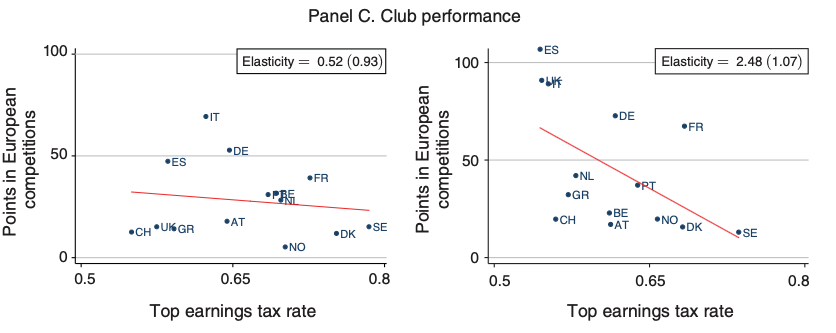
\includegraphics[
    width = \textwidth,
    keepaspectratio
  ]{bosman_1c.png}
\end{frame}

\begin{frame}{Reduced-form elasticity estimates}
\centering
\footnotesize

  {\scriptsize
\begin{threeparttable}
\begin{adjustbox}{max width=\textwidth, max height=0.5\textheight}
\begin{tabular}{lcc}
\toprule
 & \multicolumn{1}{c}{Elasticity w.r.t.\ $(1-\text{MTR})$} & \multicolumn{1}{c}{Elasticity w.r.t.\ $(1-\text{ATR})$} \\
 & (1) & (2) \\
\midrule

\multicolumn{3}{l}{\textbf{Panel A. Bosman ruling}} \\
\addlinespace[1mm]
\multicolumn{3}{l}{\textit{A1. Foreign players}} \\
Pre-Bosman  & 0.00 \,(0.86) & --- \\
Post-Bosman & 1.22 \,(0.45) & 1.79 \,(0.50) \\
\addlinespace[1mm]
\multicolumn{3}{l}{\textit{A2. Domestic players}} \\
Pre-Bosman  & 0.09 \,(0.04) & --- \\
Post-Bosman & 0.29 \,(0.08) & 0.27 \,(0.08) \\

\midrule
\multicolumn{3}{l}{\textbf{Panel B. Country case studies}} \\
\addlinespace[1mm]
\multicolumn{3}{l}{\textit{B1. Spain 2004 ``Beckham law''}} \\
Top-quality players        & 1.49 \,(0.34) & 1.87 \,(0.75) \\
Lower-quality players      & 1.43 \,(0.88) & 1.62 \,(0.82) \\
Eligible players           & 1.29 \,(0.22) & 1.41 \,(0.31) \\
Non-eligible (placebo)     & 0.57 \,(0.49) & 0.45 \,(0.78) \\

\addlinespace[1mm]
\multicolumn{3}{l}{\textit{B2. Danish tax scheme for foreigners}} \\
Top-quality players        & 3.01 \,(0.78) & --- \\
Lower-quality players      & -0.70 \,(0.54) & --- \\

\bottomrule
\end{tabular}
\end{adjustbox}

\end{threeparttable}
  }
\end{frame}

\begin{frame}{Tax Reform Case Studies}
  \begin{itemize}
    \item Compare treated country, Spain, to synthetic control created by a weighted average of the characteristics of other European countries
    \item Use a 2SLS approach to estimate elasticities:
    \begin{gather*}
      \log(P_{ct}) = e\log(1-\tau_{ct}) + \beta\mathbf{1}(c=T) + \gamma\mathbf{1}(t\geq t_0) + \varepsilon_{ct}
    \end{gather*}
    \item Instrumented with:
    \begin{gather*}
      \mathbf{1}(c=T)\times \mathbf{1}(t\geq t_0)
    \end{gather*}
    \item Estimates capture medium-term responses to reform
  \end{itemize}
\end{frame}

\begin{frame}{Beckham Law Effects}
  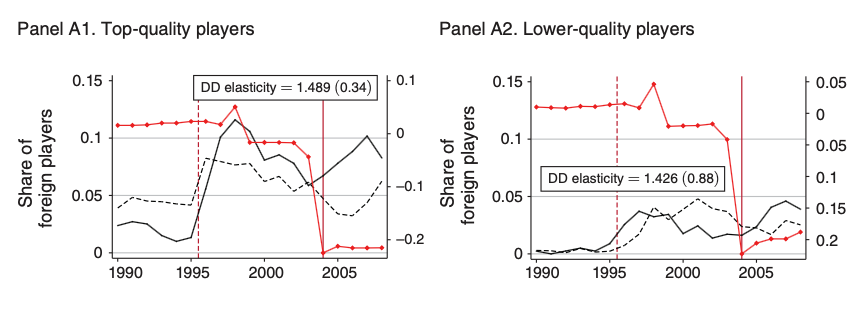
\includegraphics[
    width = \textwidth,
    keepaspectratio
  ]{beckham_1.png}
  \begin{itemize}
    \item Solid: Spain
    \item Dashed: Synthetic
    \item Red: $\Delta$ top tax rate
  \end{itemize}
\end{frame}
\begin{frame}{Beckham Law Effects, cont.}
  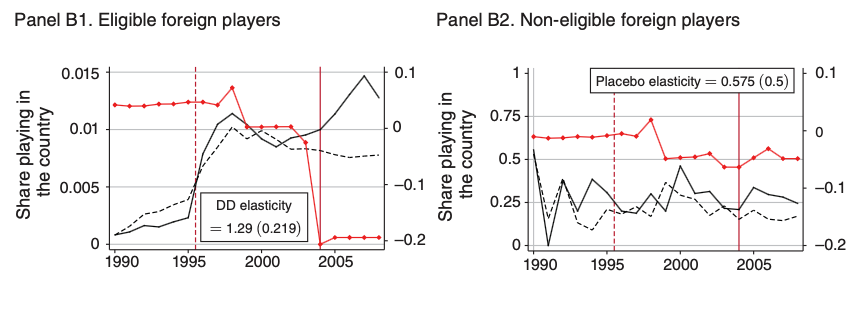
\includegraphics[
    width = \textwidth,
    keepaspectratio
  ]{beckham_2.png}
  \begin{itemize}
    \item Solid: Spain
    \item Dashed: Synthetic
    \item Red: $\Delta$ top tax rate
  \end{itemize}
\end{frame}

\begin{frame}{Danish Reform}
  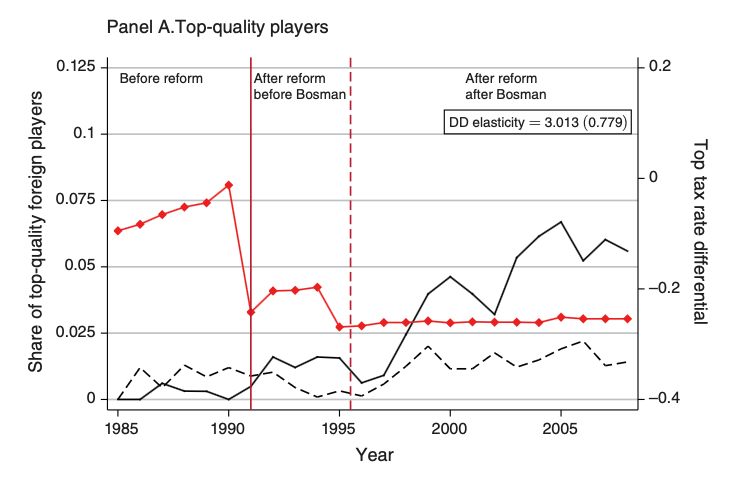
\includegraphics[
    width = 0.8\textwidth,
    keepaspectratio
  ]{denmark_1.png}
  \begin{itemize}
    \item Solid: Denmark 
    \item Dashed: Synthetic
    \item Red: $\Delta$ top tax rate
  \end{itemize}
\end{frame}

\begin{frame}{Danish Reform, cont.}
  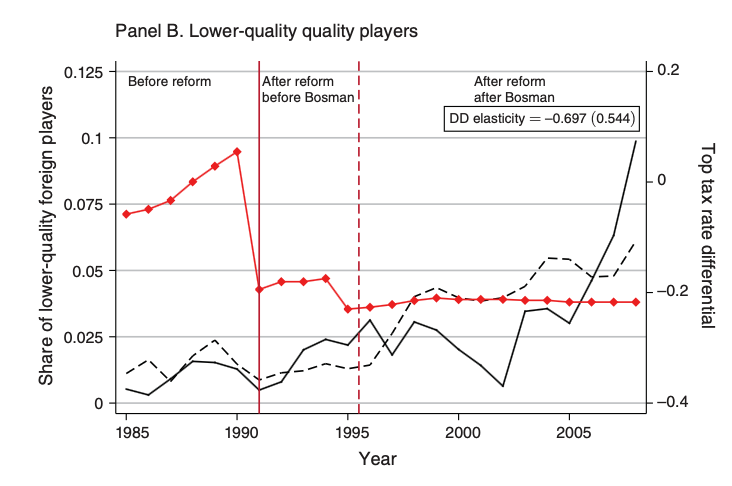
\includegraphics[
    width = 0.8\textwidth,
    keepaspectratio
  ]{denmark_2.png}
  \begin{itemize}
    \item Solid: Denmark 
    \item Dashed: Synthetic
    \item Red: $\Delta$ top tax rate
  \end{itemize}
\end{frame}

% ============================================================
\section{Empirical Estimation}
% ============================================================

\begin{frame}{Empirical Multinomial Discrete Choice}
  \begin{gather*}
    U^i_{nt} = u((1-\tau^i_{nt})w_{nt}^i) + \mu_{nt}^i \\
    = \alpha\log(1-\tau_{nt}^i) + \alpha\log(w_{nt}^i) + home_{n}^i + \mathbf{x_t^i\beta_n} + \gamma_n + \nu_{nt}^i
  \end{gather*}
  \begin{itemize}
    \item $\tau_{nt}^i$ is average tax rate on player $i$ in country $n$ at time $t$
    \item $w_{nt}^i$ is before-tax wage
    \item $\mu_{nt}^i$ idiosyncratic preference for country $n$ at time $t$ comprised of:
    \begin{enumerate}
      \item preference for home country $home_n^i$, equal to one if $n$ is the native country for player $i$
      \item individual characteristics $\mathbf{x_t^i}$ like age, age-squared. Can vary by country
      \item unobservable country specific characteristics $\gamma_n$
    \end{enumerate}
  \end{itemize}
\end{frame}

\begin{frame}{Empirical, Cont.}
  \begin{itemize}
    \item Allow $\nu_{nt}^i$ to be T1 EV $\rightarrow$ estimate Multinomial Logit
    \item Estimate first with only net-of-tax rate and home dummy as explanatory variables
    \item Add individual and country F.E.'s extension
    \item Then, contend with how to control for wage variation by:
    \begin{enumerate}
      \item Control for variation through ability channel, such that $w_{nt}^i = a_t^i$
      \item $w_{nt}^i = a_{t}^iw_{nt}$ where $w_{nt}$ captures trends in the overall market as well as cross country differences
      \item Control via country $\times$ year $\times$ ability F.E. in case of substitution between ability levels not being satisfied
    \end{enumerate}
  \end{itemize}
\end{frame}

\begin{frame}{Elasticity}
  \begin{itemize}
    \item $\alpha$ is indicative of mobility responses to net-of-tax rate
    \begin{itemize}
      \item $\alpha>0$ implies a rise in n-o-t rate leads to a positive effect on the probability of a player locating in the country
    \end{itemize}
    \item Derive probability of player $i$ locating in country $n$ w.r.t n-o-t rate in country $n$
  \end{itemize}
\end{frame}

\begin{frame}{Deriving Elasticity}
  \begin{gather*}
    P_{nt}^i = \frac{\exp\{\alpha\log(1-\tau_{nt}^i)+\mathbf{X^i_{nt}\gamma}\}}{\sum_m\exp\{\alpha\log(1-\tau_{mt}^i)+\mathbf{X_{mt}^i\gamma}\}} \\
    \varepsilon_{nt}^i\equiv\frac{d\log(P_{nt}^i)}{d\log(1-\tau_{nt}^i)} = \alpha\cdot(1-P_{nt}^i)
  \end{gather*}
  \begin{itemize}
    \item $\varepsilon_{nt}^i$ is individual elasticity of $P_{nt}^i$ w.r.t. $1-\tau_{nt}^i$
  \end{itemize}
\end{frame}
    
\begin{frame}{Deriving Elasticity, cont.}
  \hl{Domestic Elasticity:}
  \begin{gather*}
    \varepsilon_{domestic}^n = \frac{\sum_{i\in I_n}\alpha\cdot(1-P_{nt}^i)P_{nt}^i}{\sum_{i\in I_n}P_{nt}^i} = \alpha\cdot(1-\bar{P_n^d})
  \end{gather*}
  \hl{Foreign Elasticity:}
  \begin{gather*}
    \varepsilon_{foreign}^n = \frac{\sum_{i\in I_n^C}dP_{nt}^i/dlog(1-\tau_{nf})}{\sum_{i\in I_n^CP_{nt}^i}} \\
    = \frac{\sum_{i\in I_n^C}\alpha\cdot(1-P_{nt}^i)P_{nt}^i}{\sum_{i\in I_n^C}P_{nt}^i} = \alpha\cdot(1-\bar{P_n^f})
  \end{gather*}
\end{frame}

\begin{frame}{Empirical Results}
  \scriptsize
  \centering

  \begin{tabular}{lccccccc}
  \toprule
  & \multicolumn{6}{c}{Post-Bosman (1996--2008)} & Pre-Bosman \\
  & (1) & (2) & (3) & (4) & (5) & (6) & (7) \\
  \midrule
  \multicolumn{8}{l}{\textbf{Panel A. Specifications with top marginal tax rates}} \\

  \multicolumn{8}{l}{Utility parameter estimates} \\
  $\log(1-\mathrm{MTR})$
  & 1.323*** & 0.729*** & 1.089*** & 0.634*** & 1.034*** & 1.311*** & 0.202 \\
  & (0.073) & (0.116) & (0.159) & (0.132) & (0.156) & (0.139) & (0.160) \\

  \addlinespace
  \multicolumn{8}{l}{Implied elasticities} \\
  $\varepsilon_{domestic}$
  & 0.156 & 0.074 & 0.121 & 0.070 & 0.112 & 0.089 & 0.011 \\
  & (0.009) & (0.012) & (0.018) & (0.015) & (0.017) & (0.009) & (0.009) \\

  $\varepsilon_{foreigner}$
  & 1.308 & 0.704 & 1.057 & 0.621 & 0.991 & 0.747 & 0.199 \\
  & (0.072) & (0.112) & (0.154) & (0.130) & (0.150) & (0.079) & (0.158) \\
  \bottomrule
  \end{tabular}

\end{frame}

\begin{frame}{Empirical Results, Cont.}
  \scriptsize
  \centering

  \begin{tabular}{lccccccc}
  \toprule
  & \multicolumn{6}{c}{Post-Bosman (1996--2008)} & Pre-Bosman \\
  & (1) & (2) & (3) & (4) & (5) & (6) & (7) \\
  \midrule

  \multicolumn{8}{l}{\textbf{Panel B. Specifications with grouped average tax rates}} \\

  \multicolumn{8}{l}{Utility parameter estimates} \\
  $\log(1-\mathrm{ATR})$
  & 1.599*** & 0.931*** & 1.721*** & 1.123*** & 1.772*** & 1.746*** &  \\
  & (0.079) & (0.138) & (0.197) & (0.161) & (0.192) & (0.172) &  \\

  \addlinespace
  \multicolumn{8}{l}{Implied elasticities} \\
  $\varepsilon_{domestic}$
  & 0.184 & 0.093 & 0.184 & 0.122 & 0.190 & 0.116 &  \\
  & (0.009) & (0.014) & (0.021) & (0.017) & (0.021) & (0.011) &  \\

  $\varepsilon_{foreigner}$
  & 1.582 & 0.900 & 1.654 & 1.100 & 1.698 & 0.989 &  \\
  & (0.078) & (0.133) & (0.190) & (0.157) & (0.184) & (0.098) &  \\

  \addlinespace
  Country F-E
  & No & Yes & Yes & Yes & Yes & Yes & Yes \\

  Age, age squared, exp., quality $\times$ country F-E
  & No & Yes & Yes & Yes & Yes & Yes & Yes \\

  Year $\times$ country F-E
  & No & No & Yes & Yes & Yes & Yes & No \\

  Age, age squared, exp., quality $\times$ year $\times$ country F-E
  & No & No & No & Yes & No & No & No \\

  Observations
  & 55{,}225 & 55{,}225 & 55{,}225 & 55{,}225 & 55{,}225 & 55{,}225 & 45{,}577 \\

  \bottomrule
  \end{tabular}

\end{frame}


\begin{frame}{Sorting Effects, Cross-Effects, and Second Leagues (1/2)}
  \scriptsize
  \centering

  \begin{tabular}{lccccc}
    \toprule
    & (1) & (2) & (3) & (4) & (5) \\
    \midrule
    \multicolumn{6}{l}{\textbf{Panel A. Top leagues (1999--2008)}} \\
    $\log(1-\tau)$
    & 1.795*** & 1.138*** & 1.433*** &  &  \\
    & (0.065) & (0.118) & (0.155) &  &  \\
    $\log(1-\tau)\times low$
    &  &  &  & -0.512*** & -0.529*** \\
    &  &  &  & (0.149) & (0.145) \\
    $\log(1-\tau)\times top$
    &  &  &  & 1.409*** & 1.301*** \\
    &  &  &  & (0.136) & (0.132) \\
    $\log(1-\tau^f)\times domestic$
    &  &  &  &  & -0.618*** \\
    &  &  &  &  & (0.119) \\
    $\log(1-\tau^d)\times foreign$
    &  &  &  &  & -0.149 \\
    &  &  &  &  & (0.178) \\
    \bottomrule
  \end{tabular}
\end{frame}


\begin{frame}{Sorting Effects, Cross-Effects, and Second Leagues (2/2)}
  \scriptsize
  \centering
  \begin{tabular}{lccccc}
  \toprule
  & (1) & (2) & (3) & (4) & (5) \\
  \midrule
  \multicolumn{6}{l}{\textbf{Panel B. Adding the five best second leagues (1999--2008)}} \\
  $\log(1-\tau)$
  & 1.334*** & 0.995*** & 1.226*** &  &  \\
  & (0.077) & (0.128) & (0.169) &  &  \\
  $\log(1-\tau)\times low$
  &  &  &  & -0.391* & -0.448** \\
  &  &  &  & (0.158) & (0.154) \\
  $\log(1-\tau)\times top$
  &  &  &  & 1.494*** & 1.409*** \\
  &  &  &  & (0.136) & (0.133) \\
  $\log(1-\tau^f)\times domestic$
  &  &  &  &  & -0.635*** \\
  &  &  &  &  & (0.134) \\
  $\log(1-\tau^d)\times foreign$
  &  &  &  &  & -0.201 \\
  &  &  &  &  & (0.192) \\
  \addlinespace
  Country F-E
  & No & Yes & Yes & Yes & Yes \\
  Age, age squared, exp., quality $\times$ country F-E
  & No & Yes & Yes & Yes & Yes \\
  Year $\times$ country F-E
  & No & No & Yes & No & No \\
  \bottomrule
  \end{tabular}
\end{frame}

% ============================================
\section{Conclusions and Next Steps}
% ============================================

\begin{frame}{Conclusions and Takeaways}
  \begin{itemize}
    \item Mobility responses to top tax rate changes is large
    \item Elasticity on foreign players w.r.t. net-of-tax rate is about 1, even larger for top-quality foreign players
    \item Cutting taxes on foreign and local is less cost-effective than only cutting for foreign players
    \item Location elasticities are largest at the top[ and negative at the bottom, reflecting ability sorting
    \item Provide upper bound on migration response of labor market
  \end{itemize}
\end{frame}

\begin{frame}{Next Steps}
  \begin{itemize}
    \item Take framework to analyze migrate and return efficacy through football loans
    \item Potenitally applicable to human capital development $\rightarrow$ overall development as many loan players are young and looking to develop skill
    \item Utilize many data sources from this paper to get effects for footballers going on loan to get the opportunity to develop
  \end{itemize}
\end{frame}

\end{document}
